\documentclass[12pt]{standalone}
\usepackage[utf8]{inputenc}
\usepackage{tikz}
\usetikzlibrary{through}
\usetikzlibrary{intersections, calc}
\usepackage{unicode-math}
\setmathfont{Euler-Math.otf}
\def\point{1pt}
\begin{document}
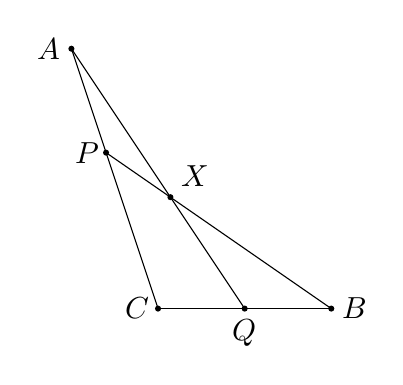
\begin{tikzpicture}[scale=1.1, transform shape]
    \coordinate [label=left:$A$] (A) at (-1,3);
    \coordinate [label=left:$C$] (C) at (0,0);
    \coordinate [label=right:$B$] (B) at (2,0);
    \coordinate [label=left:$P$] (P) at ($(A)!0.4!(C)$);
    \coordinate [label=below:$Q$] (Q) at ($(B)!0.5!(C)$);
    \fill (A) circle (\point);
    \fill (C) circle (\point);
    \fill (B) circle (\point);
    \fill (P) circle (\point);
    \fill (Q) circle (\point);

    \draw (A) -- (C);
    \draw (B) -- (C);
    \path [name path=lineBP, draw] (B) -- (P);
    \path [name path=lineAQ, draw] (A) -- (Q);

    \path [name intersections={of=lineBP and lineAQ, by={X}}];
    \node [above right] at (X) {$X$};
    \fill (X) circle (\point);
\end{tikzpicture}
\end{document}
